\chapter{RAUFlow}
\label{Capítulo 5}

% **************************** Define Graphics Path **************************
\ifpdf
    \graphicspath{{Chapter5/Figs/Raster/}{Chapter5/Figs/PDF/}{Chapter5/Figs/}}
\else
    \graphicspath{{Chapter5/Figs/Vector/}{Chapter5/Figs/}}
\fi

En cap\'itulos anteriores se ha detallado las caracter\'isticas m\'as importantes del prototipo y sus componentes. 
Resta detallar el dise\~no de la aplicaci\'on RAUFlow, encargada de implementar el plano de control del prototipo. Por ello en el presente cap\'itulo se propone un an\'alisis de dicha componente, siguiendo un proceso de dise\~no tradicional de Ingenier\'ia de Software, dividido en 4 etapas. Una primera etapa de an\'alisis de requerimientos, una segunda etapa de relevamiento de casos de uso, una tercera etapa de dise\~no del modelo de datos, y finalmente una cuarta etapa para el dise\~no general de la arquitectura de la aplicaci\'on. Ademas se presentan los aspectos m\'as importantes relacionados a la implementaci\'on de RAUFlow como por ejemplo las implementaciones del algoritmo de ruteo din\'amico y del algoritmo de distribución de etiquetas, como se implementa QoS entre otros detalles. 

\section[An\'alisi de requerimientos]{An\'alisis de requerimientos}

Anteriormente en la sección ~\ref{3.1} se definieron algunos de los requerimientos relevados para el prototipo de la RAU2. De ellos y de un trabajo de an\'alisis sobre la realidad modelada se desprende la siguiente tabla de requerimientos para RauFlow:

\clearpage
\begin{table}[Htl]\centering
\begin{tabularx}{\textwidth}{|>{\setlength\hsize{1.0\hsize}\setlength\linewidth{\hsize}}X|}
\hline
Requerimientos Funcionales\\ \hline
\hline
\begin{itemize}
\item El Sistema debe de proveer la facilidad para obtener la informaci\'on asociada a cada nodo de la red, permitiendo a su vez agregar informaci\'on que facilite la identificaci\'on del mismo para un usuario.
\item El Sistema debe proveer la facilidad para agregar, modificar y eliminar redes virtuales. 
%En particular al trabajar con redes virtuales y sus datos, se debe soportar el manejo de datos como la numeraci\'on IP del tr\'afico asociado a una red virtual, informaci\'on de capa de transporte, entre otros.
\item El Sistema debe proveer la facilidad para obtener toda la informaci\'on relevante de una red virtual.
\item El Sistema debe permitir visualizar de alguna forma los caminos constru\'idos para encaminar el tr\'afico de una red virtual en particular, a trav\'es de la red del protot\'ipo.
\item El Sistema debe proveer la facilidad para visualizar el estado de las tablas de flujos asociadas a cualquier nodo de la red del protot\'ipo.
\end{itemize}\\
\hline
\end{tabularx}
\end{table}

\begin{table}[Htl]\centering
\begin{tabularx}{\textwidth}{|>{\setlength\hsize{1.0\hsize}\setlength\linewidth{\hsize}}X|}
\hline
Requerimientos no Funcionales\\ \hline
\hline
\begin{itemize}
\item Se debe utilizar siempre que sea posible herramientas de software libre y c\'odigo abierto.
\end{itemize}\\
\hline
\end{tabularx}
\end{table}

Teniendo en cuenta la descripci\'on del problema y los requerimientos anteriores, se procedio con el modelado de la realidad. Los resultados obtenidos se presentan en la siguiente secci\'on.

%Teniendo en cuenta los requerimientos anteriores, se procede con el relevamiento de los casos de uso. Los resultados obtenidos se presentan en la siguiente secci\'on.

\section[Modelado de la realidad]{Modelado de la realidad}

Para la representaci\'on de la realidad se utiliza el paradigma de orientaci\'on a objetos. De esta forma el modelo de datos queda representado a través del siguiente diagrama de clases de diseño(ver ver figura ~\ref{fig:ModeloDeDatos}).

En el mismo se destacan en color amarillo las clases utilizadas para representar la topolog\'ia de red y sus elementos(Nodos, Interfaces y Enlaces). Cabe destacar sobre estas tres clases que en la representaci\'on asumida se busca modelar la topolog\'ia como un multigrafo dirigido. Esto se debe a que:

\begin{enumerate}
\item Tradicionalmente se utilizan grafos para el modelado de una topolog\'ia de red, siendo una representaci\'on sencilla y clara.

\item En MPLS un camino o mejor llamado LSP tiene sentido, permitiendo por ejemplo asegurar un valor de ancho de banda en un enlace para un sentido y un valor diferente para el otro sentido. Adem\'as permite establecer caminos diferentes para el tr\'afico en un sentido y en otro, priorizando por ejemplo el tr\'afico  en uno de los sentidos al utilizar el mejor camino. Utilizando grafos dirigidos puede modelarse este comportamiento.

\item En la pr\'actica nada impide que dos equipos o nodos est\'en conectados por m\'as de un enlace. De hecho este escenario es bastante beneficioso para asegurar conectividad ante la falla de enlaces. Utilizando multigrafos este escenario es modelado de forma clara.
  
\end{enumerate}

\begin{figure}[ht!] 
\centering    
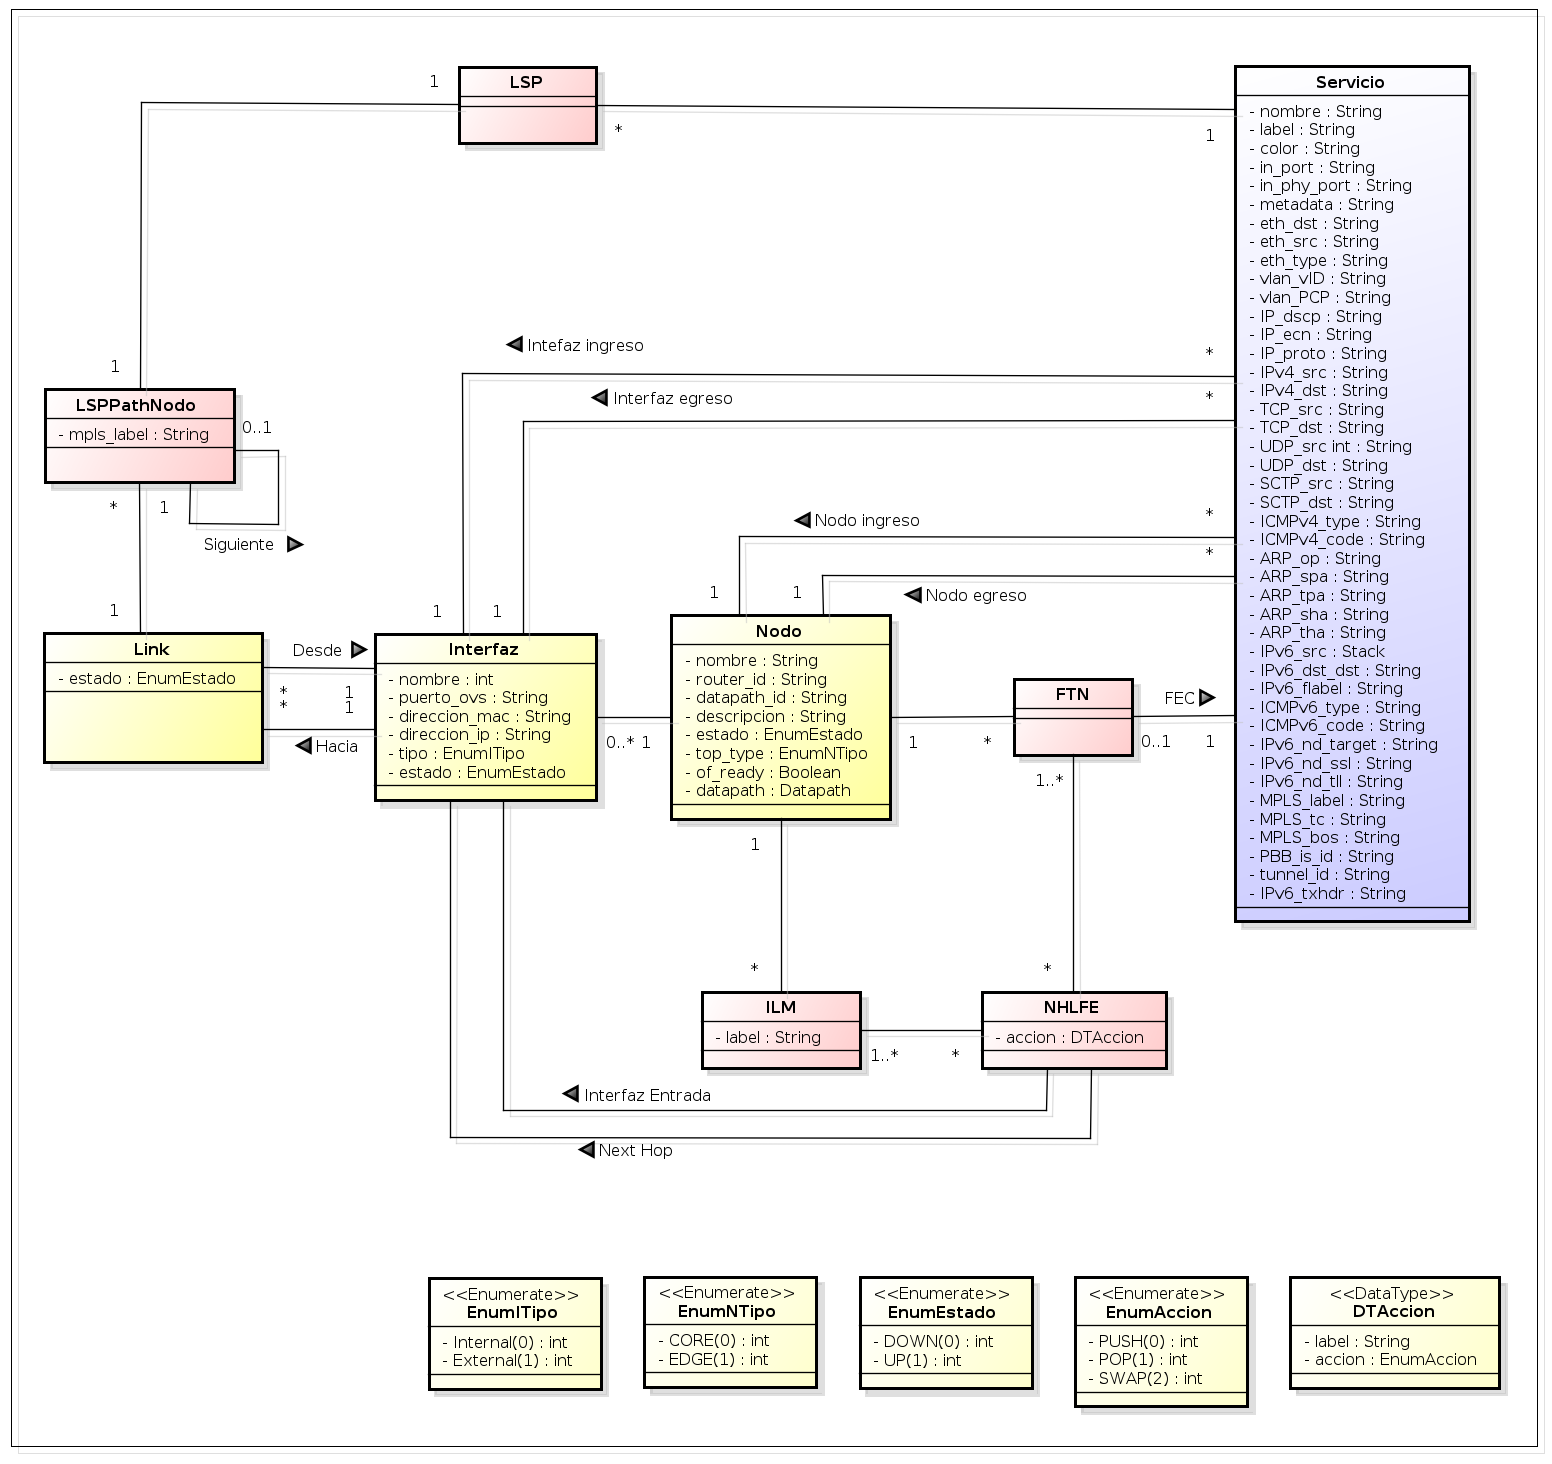
\includegraphics[width=1\textwidth]{DiagramaClases}
\caption[Modelo de datos]{Modelo de datos}
\label{fig:ModeloDeDatos}
\end{figure}

En un mulrigrafo dirigido se tienen nodos y aristas con sentido; siendo representados los nodos de una red por los nodos del grafo y los enlaces entre estos por las aristas.

En el modelo se incorpora adem\'as el concepto de Interfaz de un dispositivo. Desde entonces dos nodos presentan una arista si cada uno esta asociado a una instancia de la clase Interfaz y existe una instancia de la clase Link asociada a ambas interfaces, mediante las relaciones “Desde” y “Hacia”; indicando adem\'as estas el sentido del dicho Link.

Cabe destacar adem\'as, que en el modelo planteado no se asume que un Nodo sea f\'isicamente un dispositivo RAU-Switch; solamente se asume por simplicidad del modelo que sea un dispositivo de capa tres. Con esto se intenta contemplar la posibilidad de incorporar en un futuro adem\'as de nodos construidos en base al diseño de RAU-Switch, nodos implementados por ejemplo en base a hardware comercial.\\
  
[No se si explicar la cardinalidad 1 - * de las Interfaces - Link, la cual esta dada asi por la situacion switch dentro del core]\\

Por otro lado en rosado se destacan las clases utilizadas para representar los conceptos de la realidad relacionados a MPLS como las tablas FTN, ILM y NHLFE, y el concepto de LSP. Si bien esta \'ultima clase no tiene atributos asociados en esta versi\'on del modelo de datos, eventualmente tiene sentido en un futuro que se puedan asociar atributos del camino como el m\'aximo ancho de banda disponible y algunas otras propiedades de QoS por ejemplo.\\

Finalmente en azul se destaca el concepto Servicio, utilizado para representar un servicio de VPN provisto por un operador de red. M\'as adelante en este cap\'itulo se habla en profundidad sobre la implementaci\'on de esta clase.

Cabe destacar que por simplicidad no se representa el concepto VPN en el modelo puesto que el foco de la aplicación esta puesto en el desarrollo de los algoritmos y funcionalidades, y no en un modelado exhaustivo de la realidad. Sin embargo este concepto como muchos otros pueden ser incorporados fácilmente en un futuro.\\

Teniendo en cuenta los requerimientos mencionados, y el modelado de la realidad presentado, se procede con el relevamiento de los casos de uso. Los resultados obtenidos se presentan en la siguiente secci\'on.

\section[Relevamiento de casos de uso]{Relevamiento de casos de uso}

La lista de casos de uso presentada a continuaci\'on se corresponde con un conjunto de funcionalidades b\'asicas, que permiten la exploraci\'on de la potencialidad del enfoque SDN aplicado al problema planteado. 

\begin{itemize}
\item Listar Servicios
\item Agregar Servicio
\item Modificar Servicio
\item Eliminar Servicio
\item Ver Topolog\'ia
\item Ver informaci\'on b\'asica Nodo
\item Ver tabla de Flujos Nodo
\item Filtrar Lsps
\item Editar Informaci\'on extra Nodo
\item Editar Informaci\'on extra Interfaz
\end{itemize}

%De esta forma quedan presentados los requerimientos relevados sobre RauFlow, el modelado de la realidad, y los casos de uso relevados. Resta entonces presentar un esbozo de la arquitectura de la aplicaci\'on RauFlow, para que el lector finalmente este en condiciones de comprender el dise\~'no del prototipo en su totoalidad.
\section[Arquitectura de RauFlow]{Arquitectura de RauFlow}

En esta secci\'on se presenta la arquitectura de la aplicación RauFlow(ver figura ~\ref{fig:VistaComponentes2}), profundizándose en el funcionamiento de sus principales componentes.\\

Como se muestra en la figura\ref{fig:VistaComponentes2}, RauFlow esta basado principalmente en una aplicaci\'on Ryu(RauFlowApp) y un conjunto de aplicaciones Ryu adicionales.\\ 

Con el objetivo de mantener simple y modular el dise\~no de RauFlow, se implementa en RauFlowApp solamente aquellas funcionalidades y responsabilidades asociadas al protocolo OpenFlow y sus respectivos eventos. Luego responsabilidades y funcionalidades asociadas a la realidad modelada y sus reglas de negocios, son delegadas a una capa de negocios. Ademas se tiene un conjunto de aplicaciones Ryu dise\~nadas e implementadas por terceros, las cuales se encuentran dentro del conjunto de aplicaciones que vienen con el software Ryu. M\'as adelante se explicar\'a en detalle cual es el rol que cumplen estas aplicaciones en el dise\~no de RauFlow.

Para completar esta visi\'on general de RauFlow, se incluye en su arquitectura una interfaz de usuario gr\'afica.\\ 

En res\'umen, el dise\~no de RauFlow se caracteriza por una arquitectura en cuatro capas: (1) capa de presentación, (2) capa de aplicaciones Ryu, (3) capa de negocios, y (4) capa de dispositivos.\\

\begin{figure}[ht!] 
\centering    
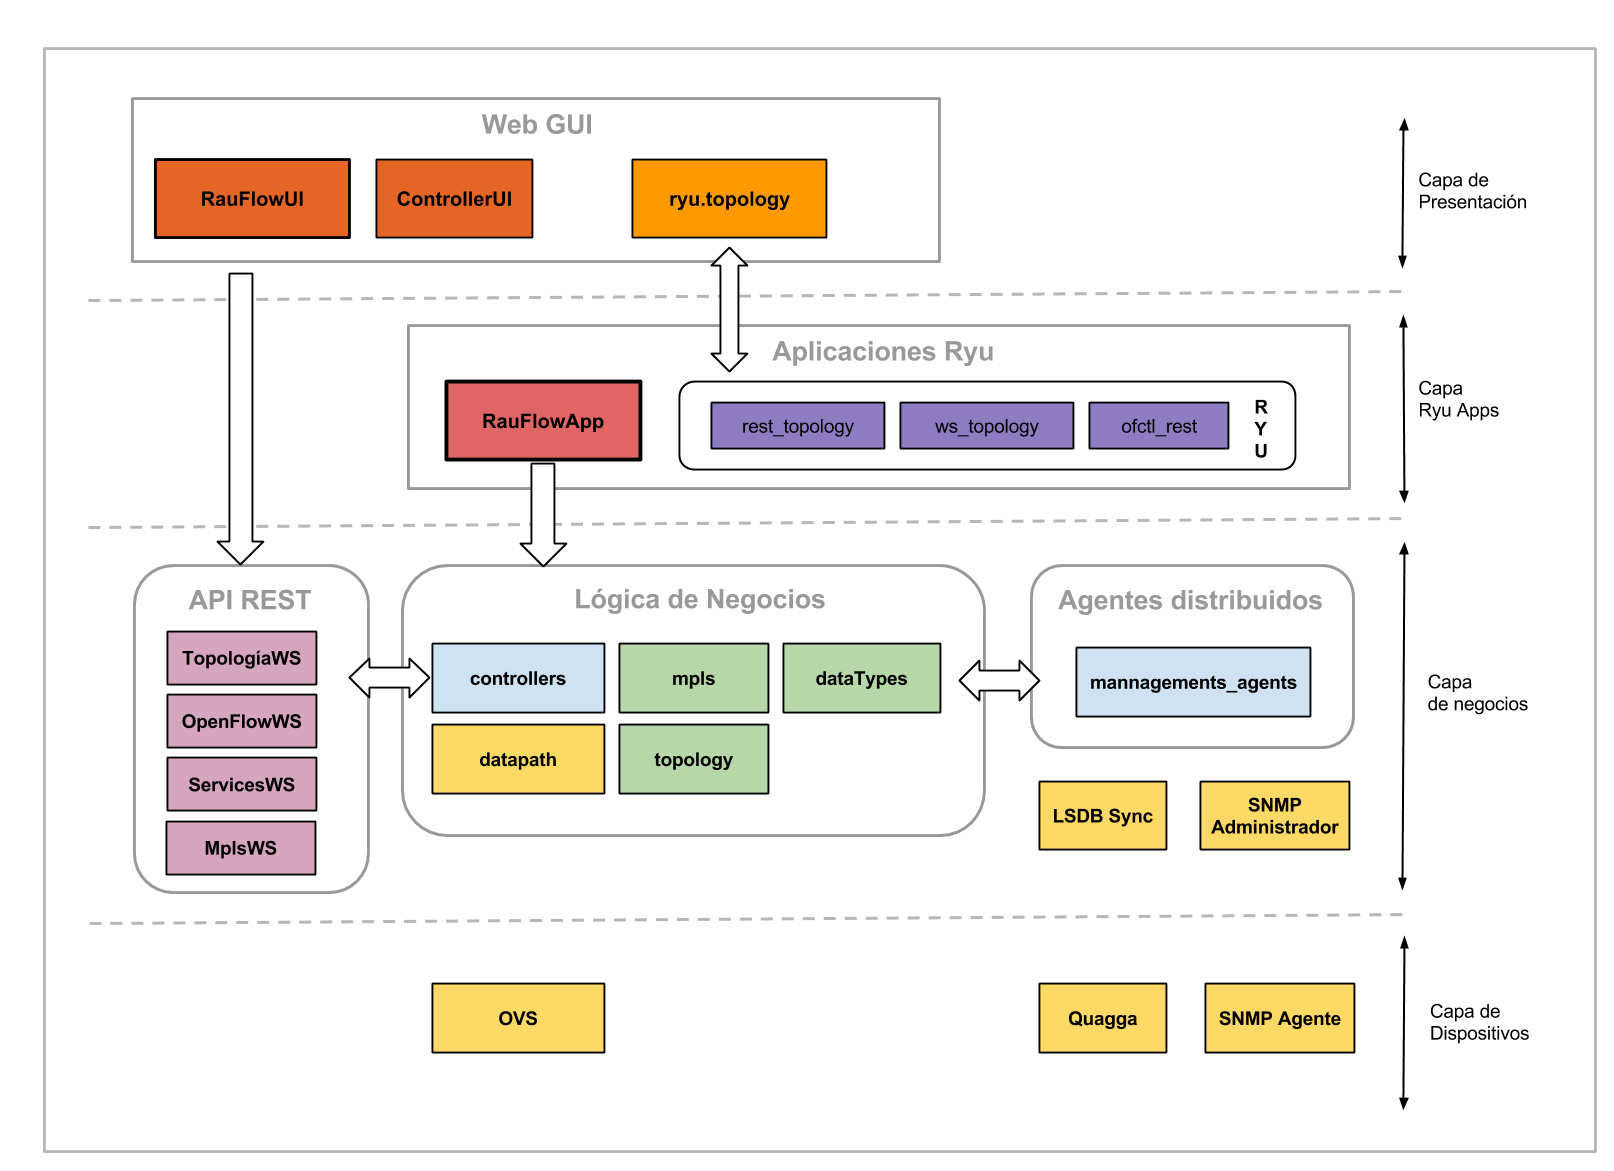
\includegraphics[width=1.0\textwidth]{Disenio_Figure3}
\caption[Vista l\'ogica]{Vista l\'ogica}
\label{fig:VistaComponentes2}
\end{figure}

\subsection{Capa de aplicaciones Ryu}
En esta capa se encuentran las diferentes aplicaciones Ryu que conforman al prototipo. Como se menciona anteriormente, RauFlow esta compuesto por una aplicaci\'on de autoria propia, y tres aplicaciones de terceros(incluidas en las aplicaciones que vienen con el software de controlador).\\

La aplicaci\'on RauFlowApp es la encargada de implementar el plano de control en el prototipo; por lo tanto, a priori su alcance puede ser tan grande como el propio alcance de RauFlow. Esto redunda en una complejidad mayor en el dise\~no de la misma. Por esta razón se decide desacoplar las reglas de negocio de la realidad, de dicha aplicación. De esta forma se genera la mencionada capa de negocios; en donde se coloca todo este conocimiento de la realidad modelada, reglas de negocio, y funcionalidades.  

\subsubsection{Aplicaciones de terceros}
Ryu incluye tres aplicaciones dise\~nadas para implementar una interfaz gr\'afica. Dicha interfaz consiste en un p\'agina web implementada sobre html, javascript y web sockets, que permite visualizar la red en su totalidad. Estos son los dispositivos del datapath con sus interfaces, y los enlaces existentes.

Por esta razon se incluyen en el dise\~no del proptotipo dichas aplicaciones, agregando funcionalidades  a la capa de presentaci\'on, y reutilizando desarrollos existentes.

\subsection{Capa de Negocios}
La capa de negocios presenta tres componentes bien definidas: una componente de reglas y l\'ogica de negocios de la realidad, una API REST de servicios para el acceso y la manipulaci\'on de datos relacionados a la primera componente, y una tercera componente denominada Agentes distribu\'idos.

\subsubsection{Lógica de Negocios}
La componente lógica de negocios se subdivide en diferentes m\'odulos que agrupan funcionalidades acorde a su naturaleza y responsabilidades. Vale la pena destacar a su vez que cada uno de estos m\'odulos se corresponde en la implementaci\'on con un package en la nomenclatura de Python. Estas funcionalidades y responsabilidades se corresponden de la siguiente forma:

\begin{itemize}
\item \textbf{controller:} Este m\'odulo agrupa diferentes controladores de objetos. Actualmente contiene un \'unico controlador façade, responsable de mantener el \'unico punto de acceso a la las componentes de la l\'ogica de negocios. Contiene desde la implementaci\'on de funciones para dar de alta Servicios, crear LSPs, obtener el mejor camino entre dos nodos de la red, etc.

\item \textbf{topology:} Agrupa las definiciones de objetos utilizados para representar la topolog\'ia como las clases Nodo, Interfaz y Link, así como otros conceptos de la realidad.
 
\item \textbf{mpls:} Contiene las definiciones de los conceptos FTN, ILM, NHLFE(rectificar esto xq esta en topology actualmente), as\'i como el conceptos de Servicio ya explicado anteriormente, y de LSP(label switched path).

\item \textbf{dataTypes:} Mantiene representaciones reducidas de los principales objetos definidos en todos los m\'odulos de la componente de negocios, para el intercambio de datos con por ejemplo la capa de presentaci\'on. 

\item \textbf{datapath:} Agrupa funcionalidades para el acceso al datapath de OpenFlow, como funciones para agregar y eliminar flujos en un switch, u obtener estad\'isticas de una tabla de flujos.
\end{itemize} 

\subsubsection{API REST de servicios}
La componente de Servicios REST, se encuentra subdividida en varios m\'odulos respondiendo al criterio utilizado para el dise\~no modular de la componente de l\'ogica de negocios. [De repente podemos poner como anexo la especificacion de la api para que se vean las funcionalidades que tiene].

\subsubsection{Agentes distribuidos}
Esta componente es la encargada de la interacci\'on con diferentes agentes y procesos instalados en cada router opensource a través de un canal de comunicación IP. Este m\'odulo de comunicaci\'on, as\'i como los diferentes agentes instalados en cada router opensource, juegan un rol irreemplazable en la obtenci\'on de informaci\'on adicional sobre cada nodo; puesto que a partir del canal de comunicaci\'on OpenFlow solamente es accesible Open vSwitch y la informaci\'on contemplada por el protocolo OpenFlow.

Dentro de esta componente, en el diagrama se muestra un modulo denominado \textbf{managements\_ agents}. Este m\'odulo opera como una interfaz de conexi\'on entre los diferentes m\'odulos de la l\'ogica de negocios, y los diferentes m\'odulos que implementan la comunicaci\'on con su respectivo agente distribu\'ido.

En la figura ~\ref{fig:VistaComponentes2} se muestran el modulo \textbf{SNMP Management}, responsable de  la comunicaci\'on con un agente SNMP distribu\'ido entre los nodos del prototipo, con el fin de obtener informaci\'on extra acerca de las interfaces de red de cada router opensource.\\

\subsection{Capa de Presentación}
Dentro de la capa de presentaci\'on se destacan: (1) una interfaz gr\'afica identificada en el esquema como RauFlowUI, la cual implementa cada uno de los casos de uso mencionados anteriormente en [link a la secci\'on de casos de uso], (2) ControladorUI, componente que funciona como nexo entre las funcionalidades de RauFlowUI y la API Rest de Servicios, y (3) \textbf{ryu.topology}. Esta \'ultima componente forma parte del conjunto de apliaciones Ryu adicionales que se incluyen en el dise\~no de RauFlow, y tiene como principal funci\'on la de proveer una representaci\'on gr\'afica en tiempo real de la topolog\'ia existente en el prototipo.\\

\section[Implementaci\'on]{Implementaci\'on}

En esta secci\'on se presentan los aspectos m\'as importantes en relaci\'on a la implementaci\'on de RauFlow. Entre ellos se destacan la implementaci\'on de la clase Servicio con la cual se implementa  clasificaci\'on de tr\'afico, el algoritmo de ruteo y el algoritmo de distribusi\'on de etiquetas.\\

\subsection{Clasificación de tr\'afico}
En la literatura de MPLS, tradicionalmente se utiliza el concepto de FEC(fordwarding equivalence class) para distinguir a un conjunto de paquetes a ser tratados en forma similar(por ejemplo para aplicar t\'ecnicas de QoS). Este concepto se define localmente a un dispositivo, determinando la forma en que un conjunto de paquetes son tratados solamente en el mismo.

En RAUFlow se aprovecha la visi\'on global del plano de control SDN para definir una noci\'on de FEC global a una topolog\'ia de red. En esta redefinici\'on se clasifica tr\'afico solamente en el nodo de ingreso a la red del prototipo, determinándose all\'i el camino a seguir por un paquete hasta el nodo de egreso. 

Este camino es calculado por el algoritmo de ruteo con restricciones(CSPF), contemplando en el políticas de ingenieria de tr\'afico y calidad de servicios. 

Por otro lado se define un mapeo entre servicio de VPN y etiquetas \textbf{mpls}, permitiendo identificar el tr\'afico asociado a un servicio en cualquier nodo intermedio de la red. Luego a partir del valor de esta etiqueta se puede realizar un procesamiento diferencial en nodos intermedios.\\

%Cuando un nuevo servicio de VPN es instanciado en RAUFlow, se ejecutan el algoritmo de ruteo para obtener el mejor camino dentro de la red, y el algoritmo de distribución de etiquetas para hallar el mapeo a etiquetas MPLS a conmutar por cada nodo del camino(LSP). Por como esta definido el algoritmo de distribución de etiquetas, este LSP es \'unico y permite identificar al servicio en cada salto por la etiqueta que se esta conmutando. De esta forma no es necesario clasificar estrictamente hablando el tr\'afico en cada nodo intermedio de la red, puesto que su camino esta dado una vez que ingresa a la red y es clasificado.

En relaci\'on a como se implementa clasificaci\'on de tr\'afico en el prototipo, se utilizan las tablas de flujos de Open vSwitch(Open vSwitch implementa 256 tablas) y los campos del cabezal OpenFlow (matching fields). Con estos campos se define las reglas de un flujo(recordar figura \ref{fig:OpenFlowArch2}) distinguiendo de este modo entre diferentes clases de tr\'afico para un procesamiento diferencial.

Dentro del cabezal OpenFlow existen campos que son para definir las reglas de un flujo y campos para definir la acci\'on de un flujo, aunque algunos de estos campos pueden utilizarse para definir ambas componentes.  

Esta lista de campos varia con la versi\'on del protocolo OpenFlow y en el contexto del prototipo esta acotada a su vez por la implementaci\'on de Open vSwitch. En el ap\'endice \ref{appendix3} se muestra  la lista entera de atributos que contiene el cabezal OpenFlow para la versi\'on 1.3 y de estos la lista de atributos que son soportados por Open vSwitch y que pueden ser utilizados para la definici\'on de reglas y acciones. Ambas listas fueron constru\'idas en base a experimentaci\'on con las herramientas Open vSwitch y Ryu.\\

En el prototipo, el concepto de clasificaci\'on de tr\'afico esta estrictamente ligado al concepto de servicio de red privada. En la siguiente secci\'on se explica la implementaci\'on es este concepto.
 
\subsection{Implementación de Servicio}

La clase Servicio, implementa en el prototipo el concepto de servicios de red privada virtual. Por tanto tiene por un lado los atributos utilizados para definir la clase de tr\'afico del servicio(campos del cabezal OpenFlow) y por otro tiene otros atributos que definen al servicio.

En el prototipo se asume que por cada nodo de borde, se tiene una \'unica red privada directamente conectada a cada interfaz externa. Esto permite definir un servicio a partir de la clase de tr\'afico definida y los pares nodo-interfaz origen, nodo-interfaz destino.

Por otro lado se puede refinar la definici\'on de servicio agregando dimensiones; una dimensi\'on bastante \'util puede ser por ejemplo el tiempo. Utilizando esta dimensi\'on, se podr\'ia por ejemplo definir un servicio de red privada par cierto horario del d\'ia o para ciertos d\'ias de la semana.

De igual forma se pueden incorporarse m\'as dimensiones orientado a brindar una mayor flexibilidad en la definici\'on de servicios, de cara a lo que podr\'ian ser diferentes requerimientos de la RAU2. 

De todos modos, teniendo en cuenta el alcance del proyecto se decidi\'o dejar las dimensiones extras como el tiempo entre otras, como una posible linea de trabajo a futuro.\\ 

%En la realidad modelada se tienen dos conceptos fundamentales asociados a un servicio de red privada virtual (VPN): (1) el concepto de clasificación de tr\'afico y (2) el concepto de calidad de servicio.\\

%En el prototipo, cuando se define un servicio se define adem\'as una clase de equivalencia de tr\'afico, en otras palabras una FEC global.



%\begin{itemize}
%\item Es un concepto global que involucra a toda la topolog\'ia
%\item Queda determinado parcialmente por la cuádrupla 
%\begin{center}
%(nodo\_ingreso, interfaz\_ingreso, nodo\_egreso, interfaz\_egreso)
%\end{center}
%\item Interesa distinguir servicios utilizando las capacidades provistas por los matching fields de OpenFlow 
%\item Esta definido temporalmente (para un rango horario espec\'ifico)[esto no se si lo ponemos]
%\end{itemize}

De esta forma se llega a la siguiente implementaci\'on de la clase servicio:\\

\begin{python}
class Service(object):

		# Atributos generales
		ID 				    # str(uuid.uuid4()) ID \'unico  
		name 				# Nombre del servicio para 
							# identificaci\'on de usuarios 
							# en RAUFlow
							
		lsps				# Lista de LSPs para el servicio
		
		ingress_node		# Nodo de ingreso del servicio
							
		egress_node 		# Nodo de egreso del servicio
							
		ingress_interface 	# Interfaz de ingreso en el nodo 
							# de ingreso
							
		egress_interface 	# Interfaz de egreso en el nodo 
							# de ingreso 
        
		# Campos del cabezal OFv1.3 
		in_port			# Switch input port. 
		metadata 		# Metadata passed between tables. 
		eth_dst 		# Ethernet destination address.
		eth_src 		# Ethernet source address. 
		eth_type 		# Ethernet frame type. 
		vlan_vID 		# VLAN id. 
		vlan_PCP		# VLAN priority. 
		IP_dscp 		# IP DSCP (6 bits in ToS field). 
		IP_ecn  		# IP ECN (2 bits in ToS field). 
		IP_proto		# IP protocol. 
		IPv4_src 		# IPv4 source address. 
		IPv4_dst 		# IPv4 destination address. 
		TCP_src 		# TCP source port. 
		TCP_dst 		# TCP destination port. 
		UDP_src 		# UDP source port. 
		UDP_dst 		# UDP destination port. 
		SCTP_src 		# SCTP source port. 
		SCTP_dst 		# SCTP destination port. 
		ICMPv4_type 	# ICMP type. 
		ICMPv4_code 	# ICMP code. 
		IPv6_src 		# IPv6 source address. 
		IPv6_dst 		# IPv6 destination address. 
		ICMPv6_type 	# ICMPv6 type. 
		ICMPv6_code 	# ICMPv6 code. 
		MPLS_label 		# MPLS label. 
		MPLS_tc 		# MPLS TC. 
		
\end{python}

En RAUFlow, cuando un nuevo servicio es creado se ejecutan los algoritmos de ruteo y distribución de etiquetas par construir un LSP. Luego este LSP es traducido a flujos OpenFlow que luego son instalados en cada uno de los nodos que forman parte. 

En la siguiente secci\'on se detalla el algoritmo de ruteo implementado en RAUFlow.

\subsection{Algoritmo de ruteo}
El algoritmo de ruteo implementado en RAUFlow parte de un algoritmo Shortest Path First(SPF) para el calculo del mejor camino entre un par de nodos en la topolog\'ia. Luego agregando restricciones al mismo es posible llegar a un Constrained Shortest Path First(CSPF) con el cual se pueda implementar funcionalidades de QoS y balanceo de carga.

En el desarrollo de este proyecto, por razones de tiempo solo fu\'e posible la implementaci\'on del algor\'iitmo SPF. De esta forma la implementaci\'on de un algoritmo de ruteo CSP partiendo del algoritmo alcanzado, se deja como una posible linea de trabajo a futuro.\\

A continuaci\'on se explica la implementaci\'on del algoritmo SPF. 

\subsubsection{Shortest Path First}
Para la construcci\'on del SPF centralizado se toma como punto de partida el algoritmo Dijkstra. Este algoritmo permite calcular en forma eficiente el mejor camino entre un par de nodos en un grafo ponderado sin costos negativos.\\

Puesto que en este trabajo se representa a una topolog\'ia de red mediante un multigrafo dirigido, es necesario o bien extender el algoritmo Dijkstra a esta representaci\'on o bien cambiar a una representación en grafos dirigidos. 

Como d representaci\'on en multigrafos dirigidos es m\'as directa e intuitivo se opta por la primera alternativa.\\

En \ref{fig:algoSPF1} se muestra el pseudo-codigo del algoritmo SPF centralizado para multigrafos dirigidos partiendo del algoritmo Dijkstra.

En el una topolog\'ia de red es representada mediante el multigrafo dirigido \textbf{G}. Las operaciones \textit{obtener\_nodos\_menor\_costo\_link} y \textit{obtener\_nodo\_adyacente\_menor\_costo} se utilizan como funciones auxiliares y se explican a continuaci\'on:

\begin{itemize}
\item obtener\_nodos\_menor\_costo\_link(w, v): Esta funci\'on permite obtener el link <w, v> de menor costo asociado en la topolog\'ia, entre los nodos w y v. Se utiliza esta operaci\'on puesto que para un par de nodos w y v pueden existir m\'ultiples links que los conecten y con diferentes costos. 

\item obtener\_nodo\_adyacente\_menor\_costo($G\setminus S$, D): Devuelve el nodo en $G\setminus S$ para el cual el costo en D de ir desde el nodo inicio a este es m\'inimo.
\end{itemize}

\begin{figure}[ht!] 
\begin{algorithm}[H]
 \SetKwFunction{CaminoMasCortoMultigrafo}{CaminoMasCortoMultigrafo} 
 \SetKwProg{myalg}{Function}{}{}
 \myalg{\CaminoMasCortoMultigrafo(G, inicio, fin){}}{\Comment{Obtiene el mejor camino en G entre los  					nodos inicio y fin, utilizando como m\'etrica el costos asociado a cada adyacencia}\\
  \textbf{Pre-condiciones:} inicio $\in$ G y fin $\in$ G\\
  \vspace{0.3cm}
  
  camino[] $\gets \lbrace\rbrace$\\														
 
  D,P $\gets$ MultiDijkstra(G, inicio, fin) \Comment{Utiliza algoritmo Dijkstra para obtener el mejor 
  													camino }\\
  i $\gets$ fin \Comment{Arma el camino en función de la lista de predecesores}\\
  \While{i $<>$ inicio}{
  	l $\gets$ P[i]\\
  	camino $\gets$ camino  $\cup$ l\\
  	i $\gets$ l.origen\\
  } 
  
  camino.Reverse()\Comment{Hay que invertir el orden del camino}\\
  
 \Return{camino}  
 }
\end{algorithm}
\caption[Algoritmo de ruteo Centralizado sin restricciones (SPF)]{Algoritmo de ruteo Centralizado sin restricciones (SPF)}
\label{fig:algoSPF1}
\end{figure}

\newpage
\begin{figure}[ht!] 
\begin{algorithm}[H]
 \SetKwFunction{MultiDijkstra}{MultiDijkstra} 
 \SetKwProg{myalg}{Function}{}{}
 \myalg{\MultiDijkstra(G, inicio, fin){}}{\Comment{Extensión de algoritmo Dijkstra para calculo de
  		mejores caminos en grafo ponderado, en un multigrafo dirigido}\\

	\vspace{0.5cm}
	
 	D $\gets \lbrace\rbrace$   \Comment{Distancias finales}\\
    P $\gets \lbrace\rbrace$  \Comment{Lista de links predecesores <nodo\_origen, nodo\_destino>}\\
    S $\gets \lbrace\rbrace$ \Comment{Lista de nodos procesados}\\
    G\_menos\_S $\gets$ G \Comment{Inicializa G $\setminus$ S como G}\\
    
    \vspace{0.2cm}
        
    S $\gets$ S $\cup$ inicio\\
    G\_menos\_S $\gets$ G\_menos\_S $- \lbrace inicio \rbrace$\\
    
    \ForEach{i in G}{
    	\If{i in G[inicio]}{\Comment{Si los nodos son adyacentes actualiza el costo en D y el link 	
    								predecesor}
    		link $\gets$ obtener\_nodos\_menor\_costo\_link(inicio, i)\Comment{Obtiene el link de 
    																	menor costo entre los nodos}\\
    		D[i] $\gets$ link.costo\\
    		P[i] $\gets$ link\\	
 		}
    }
    
    \vspace{0.2cm}

    \For{i in (1 \dots $\vert G \vert$)}{
    	w = obtener\_nodo\_adyacente\_menor\_costo(G\_minu\_S, D)\Comment{Obtiene el nodo adyacente de 	
    																		menor costo}\\
    	S $\gets$ S $\cup$ w\\
    	G\_menos\_S $\gets$ G\_menos\_S $- \lbrace w \rbrace$\\
    	\Comment{Actualiza la lista de costos y predecesores para todos los nodos en $G\setminus S$}\\
    	\ForEach{v in G\_menos\_S}{
			l $\gets$ obtener\_nodos\_menor\_costo\_link(w, v)\\
			\If{ D[w] + l.costo < D[v]}{
				D[v] $\gets$ D[w] + l.costo\\
                P[v] $\gets$ l\\
			}    	
    	}
    }
  	  
 \Return{(D, P)} 
 \vspace{1cm} 
 }
 
\end{algorithm}
\caption{SPF Centralizado continuaci\'on}
\end{figure}

\subsubsection{Constrained Shortest Path First}
 
[Aca hay que hablar de que habria que hacer para modificar el SPF y llevarlo a esto]

\subsection{Algoritmo de distribución de etiquetas}
Tradicionalmente se utilizan en \textbf{mpls} etiquetas para: (a) distinguir el tr\'afico de una VPN particular y (b) encaminar tr\'afico en la red(reenvío en base a etiquetas). De esta forma se tienen dos niveles de etiquetas usualmente denominadas inner label(para marcar el tr\'afico) y outer label(para encaminar tr\'afico - LSP).\\

Para la distribución de etiquetas(inner y outer label) existen diferentes protocolos entre los cuales puede destacarse el protocolo LDP(Label Distribution Protocol)~\citep{LDPRFC}. Este protocolo es un buen modelo de algo\'ritmo a seguir pero esta definido en base a la visión local a un nodo de la topolog\'ia red, mientras que en RAUFlow es necesario definir un algor\'itmo basado en una visi\'on global de la misma.\\

A continuaci\'on se explican los algoritmos de distribusion de etiquetas utilizados en RAUFlow para ambos niveles de etiquetas.

\subsubsection{Etiquetas internas(Inner Label)}
Mapear etiquetas mpls a servicios de VPN para posteriormente poder identificar el tr\'afico asociado dentro del prototipo es una tarea bastante simple. Una soluci\'on posible es asignar secuencialmente etiquetas dentro de un espacio de etiquetas disponible.

Esta estrategia es simple y permite crear en el sistema tantos servicios como etiquetas en el espacio disponible. Una etiqueta mpls se representa mediante 20bits $= 2^{20}$ posibles valores, lo cual si no se tienen en cuenta los valores reservados por el protocolo se pueden crear suficientes servicios con esta estrategia.\\

Si bien esta estrategia es suficiente para la asignación de la etiqueta interna, m\'as adelante en [poner link a subseccion tercer nivel de etiqueta en donde se exolica la pisadita utilizada] se ver\'a que esta estrategia es ligeramente modificada para poder soportar ciertos escenarios en el prototipo.

\subsubsection{Etiquetas externas (Outer Label)}
Asignar etiquetas a un camino \textbf{mpls} es un problema mas complejo. Aprovechando la visión global de la red puede redefinirse el algoritmo de distribución de etiquetas LDP de varias formas. Algunas de ellas pueden ser:

\begin{enumerate}
\item Asignar secuencialmente etiquetas a cada salto en un camino utilizando un espacio de etiquetas global para el LSP. De esta forma no existen dos LSPs en el sistema con etiquetas en com\'un. Esta solución tiene como ventajas su simplicidad y bajo costo en el computo del algoritmo. Por otro lado tiene como desventaja que consume el espacio de etiquetas disponibles m\'as r\'apido(hay que considerar la escala del prototipo).

\item Asignar secuencialmente etiquetas a cada salto en un camino utilizando un espacio de etiquetas global y descartando para cada interfaz etiquetas ya utilizadas por otros LSPs. Esta estrategia tiene como ventaja que es m\'as austera en el consumo de etiquetas y no existen dos LSPs con iguales etiquetas para una misma interfaz de entrada en un mismo nodo.
\end{enumerate}

Notese en relación a la segunda alternativa de implementaci\'on que debido a la forma en que se distribuyen etiquetas puede determinarse en un nodo a que servicio corresponde un paquete bas\'andse solamente en la etiqueta externa que trae y la interfaz por la que entra. Esto permite prescindir de la etiqueta interna para determinar lo que en los esquemas tradicionales se denomina FEC y aplicar eventualmente diferentes pol\'iticas de ingenier\'ia de tr\'afico, lo cual a su vez repercute en un aumento del MTU del paquete.\\ 

En RauFlow se implementa la segunda alternativa mencionada. En \ref{fig:AlgoritmoDE} se muestra el pseudoc\'odigo de una posible implementaci\'on de dicho algor\'itmo:\\

\begin{algorithm}[H]

 \SetKwFunction{obtenerEtiquetasLSP}{obtenerEtiquetasLSP} 
 \SetKwFunction{obtenerEtiquetaParaInterfaz}{obtenerEtiquetaParaInterfaz}
 \SetKwProg{myalg}{Function}{}{}
 \myalg{\obtenerEtiquetasLSP(path){}}{ \Comment{Recibe una camino en la topolog\'ia representado como 	
 												una lista ordenada de links y devuelve una lista 	
 												ordenada de etiquetas donde cada etiqueta se
 												corresponde a un link}\\
 												
    MPLS\_LABEL\_SPACE\_MIN $\gets 10$\\
 	mplsPath[] $\gets \lbrace\rbrace$\\
 	labelBase $\gets$ Null\\
 
	\uIf{len(path) = 1}{
    	$mplsPath \gets mplsPath \cup \{None\}$ \Comment{Si el camino es de largo 1, no tiene 
    													etiquetas porque primer nodo hace PHP}
 	}
 	\Else{
    	labelBase $\gets$ MPLS\_LABEL\_SPACE\_MIN \Comment{Se asignan etiquetas secuencialmente en el
    														 espacio de etiquetas}
    
   		\ForEach{l in path}{
			label $\gets$ \obtenerEtiquetaParaInterfaz(l, labelBase) \Comment{Obtiene una etiqueta 
												libre del espacio de etiquetas local a la interfaz}\\
			
			$mplsPath \gets mplsPath \cup \{label\}$\\
			
			$labelBase \gets labelBase + 1$\\
			
			$mplsPath \gets mplsPath \cup \{None\}$\Comment{Como \'ultimo nodo implementa PHP el 
													\'ultimo link no tiene etiqueta asociada}\\
				
 		}
 	}        
 
 	\Return{mplsPath[]}\;
 }
\label{fig:AlgoritmoDE}
\end{algorithm}

\newpage
\begin{algorithm}[H]
\SetKwFunction{obtenerEtiquetaParaInterfaz}{obtenerEtiquetaParaInterfaz}
\SetKwProg{myalg}{Function}{}{}
 \myalg{\obtenerEtiquetaParaInterfaz(link, label){}}{\Comment{Devuelve una etiqueta dentro del espacio de etiquetas global que no este en uso por la interfaz destino en el link. Si no existe etiqueta disponible devuelve Null}\\
 
	\vspace{0.5cm}
	 
	 etiquetas\_usadas $\gets$ link.destino.etiquetas\_usadas\\
	 next\_label $\gets$ label\_base\\
	 label $\gets$ Null\\
	 
	 \While{label is Null AND next\_label $<$ MPLS\_LABEL\_SPACE\_MAX}{
		\uIf{next\_label in etiquetas\_usadas)}{
    		next\_label $\gets$ next\_label + 1\\
    	}
 		\Else{
 			label $\gets$ next\_label\\
 		}
	 }
	 
	\If{label $<>$ Null)}{
     	link.destino.etiquetas\_usadas $\gets$ link.destino.etiquetas\_usadas $\cup$ label\\
	}
	
	\Return{label}
 }
 
  \caption{How to write algorithms}
\end{algorithm}

\subsubsection{Stack de etiquetas MPLS}
Se le denomina stack de etiquetas mpls a la pila de etiquetas que resulta de superponer una etiqueta sobre otra en un paquete. Al inicio de esta secci\'on se menciona la utilizaci\'on de dos niveles de etiquetas, una etiqueta interna para identificar el servicio y una etiqueta externa para marcar el camino dentro de la red del prototipo. Luego cuando se describe la implementaci\'on del algoritmo de distribución de etiquetas de segundo nivel(etiquetas externas), se muestra que es posible prescindir del primer nivel de etiquetas(etiquetas internas).\\

Por un lado puede implementarse el prototipo trabajando solamente con un nivel de etiquetas, garantizando reenvío en base a etiquetas y clasificaci\'on de tr\'afico. Sin embargo para poder identificar el servicio asociado a un paquete en el nodo de egreso en un LSP, es necesario que el paquete presente la etiqueta correspondiente; permitiendo de esta forma reenviarlo por la correcta interfaz de salida del prototipo. 

Esto no es posible si se implementa Penultimate Hop Popping(PHP) dado que la etiqueta es removida en el pen\'ultimo hop, llegando al nodo de egreso sin etiquetas.

Pensando en permitir en un futuro la conexi\'on al prototipo de nodos diferentes a RAU-Switch, eventualmente de hardware comercial, es necesario mantener la implementaci\'on estándar de \textbf{mpls}, debiendo implementar PHP obligatoriamente.

Teniendo en cuenta las ventajas y desventajas de ambas alternativas, se decide implementar PHP y trabajar con dos niveles de etiquetas como se plantea inicialmente.\\

Anteriormente en esta secci\'on se mencion\'o la necesidad de modificar el algoritmo de distribución de etiquetas de primer nivel por un problema particular. A continuaci\'on se explica el escenario que origina este problema y su soluci\'on.\\

En una red MPLS cada vez que un paquete es manipulado para colocar un cabezal mpls, el ethertype del paquete original es sustituido por el del protocolo. Por otro lado cuando la etiqueta de primer nivel es removida en el nodo de egreso se debe colocar el ethertype original del paquete. 

Mientras que en un servicio de VPN de capa 3 este problema puede resolverse definiendo servicios específicos por ethertype, en una VPN de capa 2 es necesario recurrir a otro tipo de soluciones.

Es necesario entonces guardar en alg\'un lado el valor original de ethertype para cada paquete que ingresa al prototipo y colocarlo en el \'ultimo nodo del camino, si se quiere soportar la implementacion de VPNs de capa 2 en el prototipo. Esto puede realizarse al menos de las siguientes dos formas:

\begin{enumerate}
\item Cada paquete que ingresa a la red del prototipo es enviado al Controlador en donde se extrae y guarda el valor original de ethertype. Luego se continua con el procesamiento del paquete acorde a las reglas ya definidas. Luego cuando el paquete arriba al ultimo nodo, tras procesarse acorde a las reglas ya definidas(extraer etiqueta de primer nivel por ejemplo) el paquete es enviado al Controlador donde se le coloca el valor original de ethertype. Finalmente se reenv\'ia el paquete por la interfaz de salida de la red del prototipo.

Este soluci\'on se corresponde con un enfoque reactivo de red SDN (recordar estado del arte en las redes definidas por software).

\item Se utilizan etiquetas para indicar el ethertype de un paquete. Se puede definir un tercer nivel de etiquetas para esto, definiendo un mapeo entre ethertype y etiqueta. Luego el nodo de egreso utilzando esta informaci\'on sabe localmente que ethertype colocar en el paquete antes de reenviarlo por la interfaz de salida. 

Por otro lado no es bueno utilizar un tercer nivel de etiquetas a menos que sea extrictamente necesario ya que esto agrega complejidad al procesamiento del paquete y reduce el MTU. 

Una alternativa mejor es utilizar el primer nivel de etiquetas para identificar el ethertype, definiendo para cada servicio de VPN en vez de una etiqueta un rango de etiquetas(una etiqueta para cada tipo de ethertype soportado). De esta forma se pueden definir flujos para cada servicio y cada ethertype en el nodo de egreso, para colocar nuevamente el ethertype original dependiendo del valor en la etiqueta de primer nivel. 

\end{enumerate} 

\subsection{Ciclo de vida de un Nodo}

En el prototipo se obtiene informaci\'on de varias fuentes de datos para la construcci\'on de la topolog\'ia. Algunas de ellas son la base de datos topol\'ogica de Quagga(LSDB), el datapath OpenFlow y a través del ingreso manual de informaci\'on mediante la interfaz gr\'afica de RAUFlow.

Estas fuentes aportan datos en forma independiente, lo cual incide directamente en la construcci\'on de la topolog\'ia y en decisiones que se toman dentro del prototipo como por ejemplo en el algoritmo de ruteo entre otros. Por ello a contnuaci\'on se ejemplifica el proceso de construcci\'on de la topolog\'ia a partir de las fuentes de datos, tomando como ejemplo el ciclo de vida de un nodo en particular. Luego el ciclo de vida de interfaces y enlaces puede deducirse de forma análoga.\\

\begin{figure}[ht!] 
\centering    
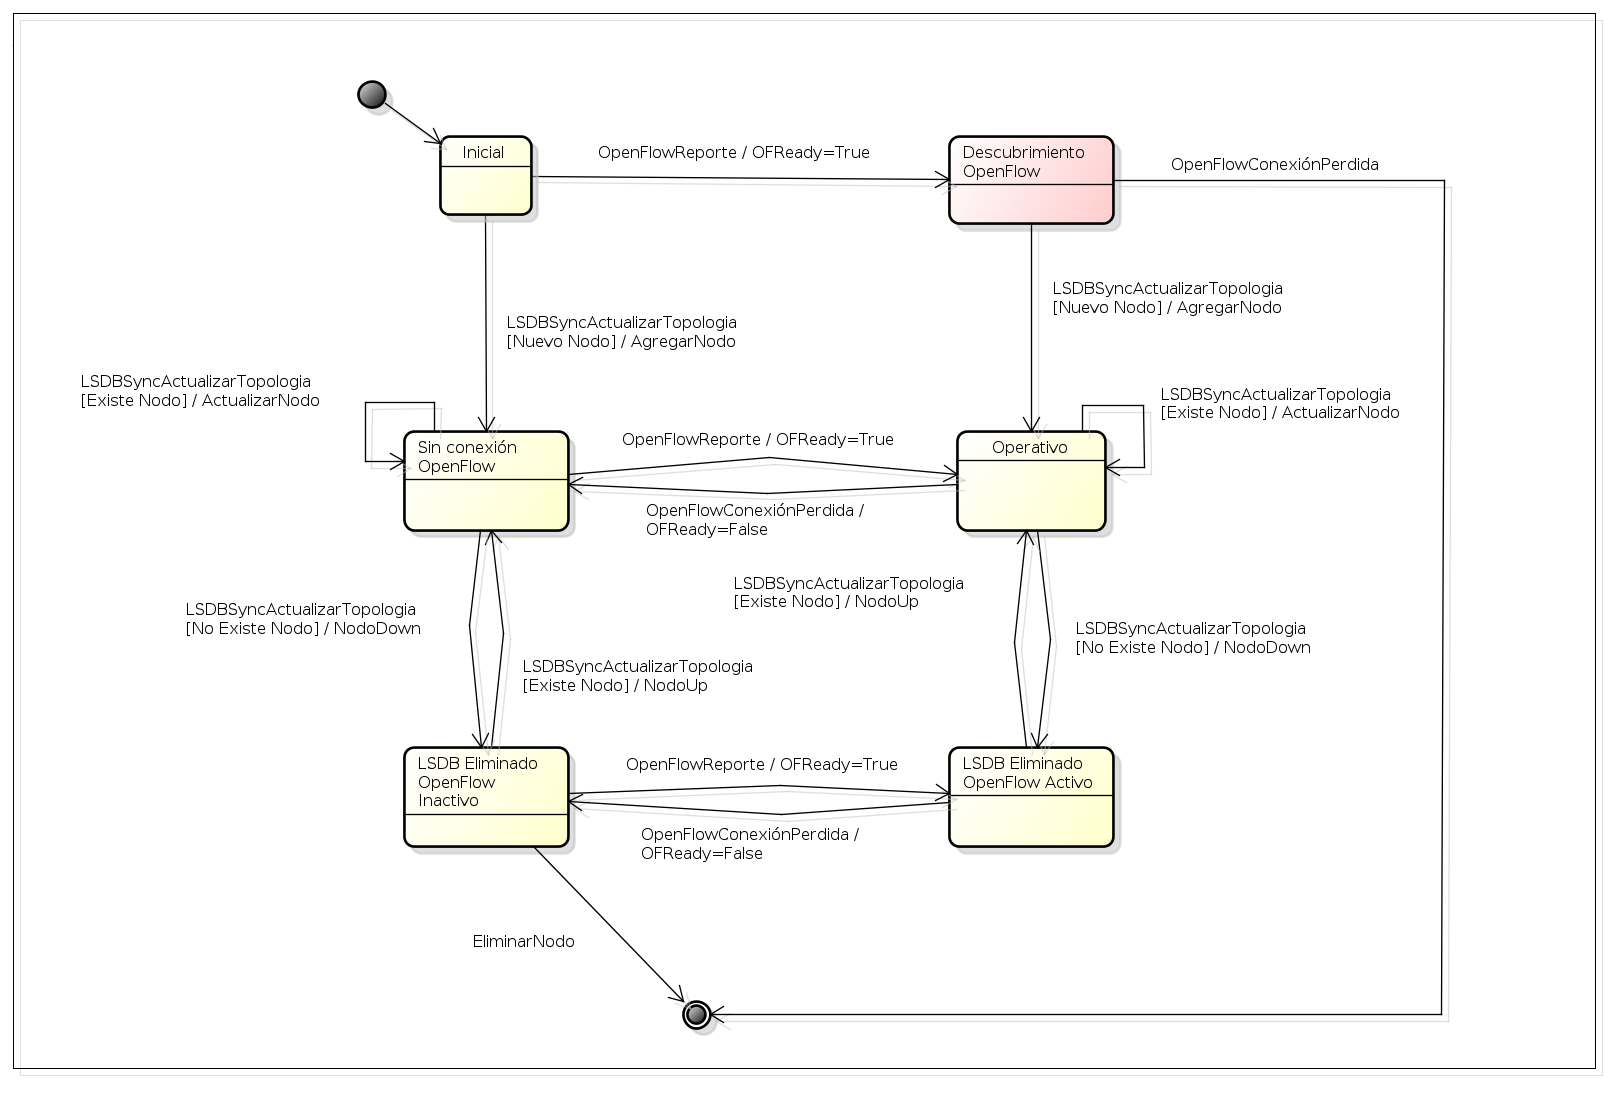
\includegraphics[width=1\textwidth]{CicloVidaNodo2}
\caption[Ciclo de vida de un Nodo]{Ciclo de vida de un Nodo}
\label{fig:CicloVidaNodo}
\end{figure}
  
Como se muestra en la figura\ref{fig:CicloVidaNodo}, despreciando el estado inicial un Nodo presenta cinco estados diferentes en el sistema: \textit{Descubrimiento OpenFlow}, \textit{Sin Conexión OpenFlow}, \textit{Operativo}, \textit{LSDB Eliminado OpenFlow Inactivo} y \textit{LSDB Eliminado OpenFlow Activo}.\\

A continuación se explica cada uno de los estados, así como las posibles transiciones:

\begin{itemize}
\item \textit{Descubrimiento OpenFlow:} Cuando un switch se reporta mediante el protocolo OpenFlow por primera vez con el Controlador y en este caso con RAUFlow, se guarda diferente informaci\'on del mismo y en particular la instancia de la clase Datapath asociada a la implementaci\'on de Ryu(esta instancia es utilizada posteriormente para interactuar con el dispositivo). Si el switch OpenFlow no esta instanciado como Nodo en el sistema, entonces se almacena en una lista temporal de Nodos. Por una decisión de diseño no se crea una instancia del Nodo como tal, logrando de esta forma que el mismo no sea considerado por el prototipo en ninguna de las funcionalidades y algoritmos implementados (no se muestra a través de la GUI, no es considerado en el algoritmo de ruteo, etc). 

Este estado representa esta situación. De el pueden suceder dos cosas, que el switch deje de reportarse con el controlador en cuyo caso es eliminado de la lista temporal de Nodos o que la componente LSDBSync envíe una actualizaci\'on de la topolog\'ia, en donde se incluye el nodo en cuestión. En este caso se instancia un objeto Nodo con toda la informaci\'on provista por la LSDB(Link State Database de Quagga), datapath de OpenFlow y la inormaci\'on adicional obtenida con el agente SNMP, y el Nodo cambia al estado \textit{Operativo}.

Vale la pena destacar que en caso de no poder obtener la informaci\'on adicional con el agente SNMP, el Nodo no es instanciado y se mantiene en el estado actual.

\item \textit{Operacional:}

Este estado es utilizado para representar a aquellos nodos que se encuentran en la LSDB y fueron rectificados o instanciados en la \'ultima actualizaci\'on de la topolog\'ia, y a su vez se encuentran report\'andose mediante el protocolo OpenFlow.

En este estado el nodo es mostrado por la interfaz gr\'afica de RAUFlow, y se tiene acceso a todas las características del mismo, tanto del modelo de datos presentado como las que son accesibles a trav\'es del datapath. Adem\'as es considerado para el calculo de las mejores rutas, y puede ser utilizado como nodo de ingreso \'o egreso en la definici\'on de servicios.

En pocas palabras es un nodo completamente funcional a los efectos de la implementaci\'on de RAUFlow.

Desde este estado se tienen tres transiciones posibles. Una primera posibilidad es que se produzca una actualización de la LSDB(evento LSDBSyncActualizarTopologia) y que en la topolog\'ia recibida se encuentre el Nodo en cuesti\'on. En este caso solamente se actualiza la informaci\'on asociada al nodo(acción ActualizarNodo), entre la cual se incluye la actualización de las Interfaces y Links, quedando en el estado actual. Una segunda posibilidad es que el switch deje de reportarse por el canal OpenFlow(evento OpenFlowConexiónPerdida) en cuyo caso se modifica el atributo of\_ready del Nodo asignando el valor False, y se cambia al estado \textit{Sin Conexión OpenFlow}. Por \'ultimo una tercera posibilidad es que se produzca una actualizaci\'on de la LSDB(evento LSDBSyncActualizarTopologia) y que el Nodo no este en la topolog\'ia recibida. En este caso se cambia el valor del atributo estado en el Nodo(NodoDOWN), asignandose el valor 0 que se corresponde con el estado DOWN, y se cambia al estado \textit{LSDB Eliminado OpenFlow Activo}.

\item \textit{LSDB Eliminado OpenFlow Activo:} Este estado contempla a un Nodo que no se encontraba en la LSDB recibida en la ultima actualizaci\'on topol\'ogica pero que a\'un se reportan por el canal de comunicaci\'on OpenFlow.

Desde este estado se tienen solamente dos transiciones posibles. Una primera posibilidad es que se produzca nuevamente una actualización de la topolog\'ia 
(LSDBSyncActualizarTopologia) y que el nodo se encuentre dentro de la información recibida. En este caso se actualiza el estado del nodo(NodoUP) y se cambia al estado \textit{Operativo}. Una segunda posibilidad es que el nodo deje de reportarse por el canal OpenFlow(OpenFlowConexiónPerdida) en cuyo caso se actualiza el valor del atributo of\_ready al valor False y se cambia al estado \textit{LSDB Eliminado OpenFlow Inactivo}.

\item \textit{Sin Conexión OpenFlow:} Este estado contempla a un Nodo que fue creado o rectificado en la \'ultima actualización de la LSDB pero que no se ha reportado por el canal OpenFlow; ya sea porque nunca lo hizo o porque dejo de hacerlo. En este estado el Nodo es mostrado a trav\'es de la interfaz gr\'afica de RAUFlow pero no es considerado ni para el el calculo de mejores caminos ni para la creaci\'on de nuevos servicios tanto como nodo de ingreso \'o egreso. Adem\'as la informaci\'on asociada al datapath de OpenFlow como las tabla de flujos y estad\'isticas tampoco son accesibles.

De este estado existen tres transiciones posibles. Por un lado el nodo puede estar presente en la LSDB al producirse una actualizaci\'on de la topolog\'ia(LSDBSyncActualizarTopologia), actualizandose la informaci\'on del nodo(ActualizarNodo) y manteniéndose en el mismo estado. Por otro lado tambi\'en al producirse una actualizaci\'on de la topolog\'ia, el nodo puede no estar en la LSDB, en cuyo caso se actualiza el estado del nodo(NodoDOWN) y se cambia al estado \textit{LSDB Eliminado OpenFlow Inactivo}. Finalmente el switch puede empezar a reportarse por el canal OpenFlow(OpenFlowReport) en cuyo caso se actualiza el valor del atributo of\_ready a True, y se cambia al estado \textit{Operativo}.  

\item \textit{LSDB Eliminado OpenFlow Inactivo:} Este estado modela a un Nodo que nunca se reporto \'o dej\'o de reportarse por el canal OpenFlow, y que a su vez no se encuentra dentro de la LSDB en la \'ultima actualizaci\'on topol\'ogica realizada. De este estado existen tres transiciones posibles.

Una primera alternativa es que el switch en cuesti\'on se reporte con la aplicaci\'on(OpenFlowReporte), en cuyo caso se actualiza el valor del atributo of\_ready a True y se cambia el estado a \textit{LSDB Eliminado OpenFlow Activo}. Una segunda alternativa es que se produzca una actualizaci\'on de la topolog\'ia y el Nodo se encuentre dentro de la LSDB, en cuyo caso se cambia el estado del nodo(NodoUP) y se cambia al estado \textit{Sin conexión OpenFlow}. Finalmente una tercera alternativa es que el nodo  sea eliminado del sistema. Si bien esta funcionalidad no se encuentra actualmente implementada, la idea es que un Nodo para el cual no se ha recibido reportes por el canal OpenFlow luego de un tiempo determinado, y que tampoco aparece en la LSDB tras una actualicaci\'on, pueda ser eliminado del sistema, eventualmente tras la intervenci\'on de un usuario administrador mediante la interfaz gr\'afica.
  
\end{itemize}

El ciclo de vida de una Interfaz \'o un Link puede ser explicado de forma an\'aloga con una m\'aquina de estados similar, teniendo presente las relaciones existentes entre las tres clases, Nodos, Interfaces y Links.

\newpage
\subsection{Actualizaci\'on de la topologia}

\newpage
\begin{algorithm}[H]
 \SetKwFunction{UpdateServicesLSPs}{UpdateServicesLSPs} 
 \SetKwProg{myalg}{Function}{}{}
 \myalg{\UpdateServicesLSPs(){}}{
    Declare  mpls\_tables\_ftn $\gets \{\}$\\
    Declare  mpls\_tables\_ilm $\gets \{\}$\\
 	\ForEach{n in topology}{
 		 mpls\_tables\_ilm[n.router\_id] $\gets$ n.ilm\\
         n.ilm $\gets []$\\
         
         mpls\_tables\_ftn[n.router\_id] $\gets$ n.ftn\\
         n.ftn $\gets []$\\
         
         n.nhlfe $ \gets []$\\		
 	}
 	\ForEach{s in services}{
 		lsps\_nuevos $\gets$ []\\
 		
 		\ForEach{lsp in s.lsps}{
 			lsp\_nuevo $\gets$ update\_lsp(s, lsp)\\
            lsps\_nuevos $\gets$ lsps\_nuevos $\cup$ lsp\_nuevo\\
 		}
 		
 		s.lsps $\gets$ lsps\_nuevos	
 	}
 	\ForEach{n in topology}{
 	ftn\_adds $\gets \lbrace$ n.ftn $\rbrace$ - $\lbrace$ mpls\_tables\_ftn[n.router\_id]$\rbrace$\\
    ftn\_removes $\gets \lbrace$ mpls\_tables\_ftn[n.router\_id]$\rbrace$ - $\lbrace$ n.ftn $\rbrace$\\
    ilm\_adds $\gets \lbrace$ n.ilm $\rbrace$ - $\lbrace$ mpls\_tables\_ilm[n.router\_id] $\rbrace$\\
	ilm\_removes $\gets \lbrace$ mpls\_tables\_ilm[n.router\_id]$\rbrace$ - $\lbrace$ n.ilm $\rbrace$\\		
	\ForEach{ftn in ftn\_removes}{
		service $\gets$ ftn.service\\
		remove\_egress\_node\_service\_flows(service, n, ftn)\\
	}
	\ForEach{ilm in ilm\_removes}{
		\ForEach{nhlfe in ilm.nhlfes}{
			remove\_node\_service\_flow(n, ilm, nhlfe)\\
		}
	}
	\ForEach{ftn in ftn\_adds}{
		service $\gets$ ftn.service
		install\_ingress\_node\_service\_flows(service, n, ftn)\\
	}
	\ForEach{ilm in ilm\_adds}{
		\ForEach{nhlfe in ilm.nhlfes}{
	
			\uIf{next\_hop.i\_type == 1}{\Comment{Si el tipo de interaz es 1 entonces es un nodo de borde y el flujo es diferente}\\
    			install\_egress\_node\_flow\_for\_service(service, n, ilm, nhlfe)\\	
 			}

 			\Else{
 				\Comment{Es un nodo interno entonces el flujo es normal}\\
 				install\_node\_flow\_for\_service(n, ilm, nhlfe)
 			}
		}
	}	
 	}  	
 }  
 \caption{Algoritmo de actualización de la topolog\'ia}
\end{algorithm}

\newpage
\subsection{Implementaci\'on de QoS}
\label{5.5.4}



\newpage
\subsubsection{SPF}
asdasd

\newpage
\subsubsection{CSPF}
Dijkstra para multi grafos dirigidos.

[AYUDA MEMORIA: Cosas de las que hay que hablar]

\begin{itemize}
\item SPF y CSPF: Mostrar el pseudo codigo del algoritmo de ruteo implementado, mencionar que esta construido sobre dijkstra para multigrafos. En particular mencionar que cosas de QoS interesaria meter en este algoritmo para garrantizar QoS despues en RauFlow

\item Mencionar como se implementaria QoS en RauFlow

\item Capaz algo sobre la interfaz 
\end{itemize}
